%---------------------------------------------------------------------
%   documentclass
%---------------------------------------------------------------------
\documentclass[a4paper]{article}

%---------------------------------------------------------------------
%   packages
%---------------------------------------------------------------------

\usepackage[english]{babel}
\usepackage[enc=cp1250]{hrlatex}

\usepackage{algorithmic}
\usepackage{algorithm}
\usepackage{amsmath}
\usepackage{amsthm}
\usepackage[titletoc, page]{appendix}
\usepackage{booktabs}% http://ctan.org/pkg/booktabs
\usepackage{bm}
\usepackage{caption}
\usepackage{cite} %bibtex
\usepackage{color} %for \definecolor
\usepackage{colortbl} %for \rowcolor command
\usepackage{courier}
\usepackage{enumitem}
\usepackage{eucal} %for nice letters like \mathcal{A}
\usepackage{floatflt} %to have tables and text beside
\usepackage[T1]{fontenc} %pekne makcene
\usepackage{hyperref} %odkazy
\usepackage{listings}
\usepackage{lmodern} %spolu s T1 smooth font!
\usepackage{lscape}
\usepackage{mathtools}
\usepackage{multirow}% http://ctan.org/pkg/multirow
\usepackage{pdfpages}
\usepackage{pgfplots}
\usepackage{pifont} %for ticks (check symbols)
\usepackage{scalefnt}
\usepackage{setspace}
\usepackage{subcaption}
\usepackage{tikz}
\usepackage{titlesec} %section titles font size change
\usepackage{xcolor} %for \colorlet

\usetikzlibrary{decorations.pathreplacing}

%---------------------------------------------------------------------
%   margins
%---------------------------------------------------------------------
\oddsidemargin 0.3in
\evensidemargin 0.3in
\textwidth 6in
\textheight 23.5cm
\topmargin -0.35in

\linespread{1.2}
\renewcommand{\arraystretch}{1.1} %spacing of table rows

%---------------------------------------------------------------------
%   various settings
%---------------------------------------------------------------------
\newif\ifmine % introduce a switch for draft vs. final document
\minetrue

\newif\iffinal % introduce a switch for draft vs. final document
\finaltrue % use this to compile the final document
\iffinal
  \newcommand{\inputTikZ}[1]{%
    \input{#1.tikz}%
  }
\else
  \newcommand{\inputTikZ}[1]{%
    \beginpgfgraphicnamed{#1-external}%
    \input{#1.tikz}%
    \endpgfgraphicnamed%
  }
\fi

\setlist{nolistsep} %so that lists have normal spacing

\titleformat{\section}{\LARGE\bfseries}{\thesection}{1em}{} %section titles
\titleformat{\subsection}{\Large\bfseries}{\thesubsection}{1em}{} %subsection titles

\definecolor{tablehead}{RGB}{238,233,233} %nice smooth grey
\definecolor{algcolor}{RGB}{0,0,0}
\definecolor{inalgcolor}{RGB}{0,0,0}
\definecolor{lstcolor}{RGB}{238,233,233}

\setlength{\parindent}{0pt} %we don't need no indentation

\graphicspath{{./pics/}} %picture dir

\lstset{ %
    language=Octave,                % choose the language of the code
    basicstyle=\footnotesize\ttfamily,       % the size of the fonts that are used for the code
    numbers=left,                   % where to put the line-numbers
    numberstyle=\footnotesize,      % the size of the fonts that are used for the line-numbers
    stepnumber=1,                   % the step between two line-numbers. If it's 1 each line will be numbered
    numbersep=5pt,                  % how far the line-numbers are from the code
    backgroundcolor=\color{lstcolor},   % choose the background color. You must add \usepackage{color}
    showspaces=false,               % show spaces adding particular underscores
    showstringspaces=false,         % underline spaces within strings
    showtabs=false,                 % show tabs within strings adding particular underscores
    frame=single,	                % adds a frame around the code
    tabsize=2,	                    % sets default tabsize to 2 spaces
    captionpos=b,                   % sets the caption-position to bottom
    breaklines=true,                % sets automatic line breaking
    breakatwhitespace=false,        % sets if automatic breaks should only happen at whitespace
    title=\lstname,                 % show the filename of files included with \lstinputlisting; also try caption instead of title
    escapeinside={\%*}{*)},          % if you want to add a comment within your code
%    morekeywords={*,...}            % if you want to add more keywords to the set
	deletekeywords={all, null, length, path, function}
}

\colorlet{city-clr}{green!70!black}
\colorlet{elcon-clr}{red}
\colorlet{event-clr}{blue}
\colorlet{waiting-clr}{olive}
\colorlet{cmt-clr}{gray}
\colorlet{oracle-clr}{orange!30}
\colorlet{algsec-clr}{black!50!red}

%---------------------------------------------------------------------
%   environments
%---------------------------------------------------------------------
\renewenvironment{abstract}[1]
{
	\Large
	\begin{center}
		\textbf{#1}
	\end{center}
	
	\normalsize
	
	\addtolength{\leftskip}{1in}
	\addtolength{\rightskip}{1in}
	\setlength{\parindent}{0in}
}
{
}

\newenvironment{itemizesp}
{
    \begin{itemize}
}
{
    \end{itemize}
}

\newcommand{\cmt}[1]{{\color{cmt-clr} \hspace*{1cm} \# \textit{#1}}}
\newcommand{\algsec}[1]{\textcolor{algsec-clr}{\textbf{\underline{#1}}}} 
\newcommand{\deftoken}{\boldmath{$\mathcal{DEFINITION}$}}
\newcommand{\restoken}{\boldmath{$\mathcal{RESULT}$}}
\newcommand{\dotoken}{\boldmath{$\mathcal{DO METHOD}$}}
\newcommand{\textbff}[1]{{\large \textbf{#1}}}
\newcommand{\tick}{\ding{52}}
\newcommand{\cross}{\ding{55}}

\numberwithin{figure}{section}
\numberwithin{table}{section}
\numberwithin{equation}{section}

\newtheorem{definition}{Definition}[section]
\newtheorem{example}{Example}[section]
\newtheorem{theorem}{Theorem}[section]
\newtheorem{lemma}{Lemma}[section]
\newtheorem{observation}{Observation}[section]

\interfootnotelinepenalty=10000

%---------------------------------------------------------------------
%   magic code
%---------------------------------------------------------------------
% Here it is: the code that adjusts justification and spacing around caption.
\makeatletter
% http://www.texnik.de/floats/caption.phtml
% This does spacing around caption.
\setlength{\abovecaptionskip}{6pt}   % 0.5cm as an example
\setlength{\belowcaptionskip}{6pt}   % 0.5cm as an example
% This does justification (left) of caption.
\long\def\@makecaption#1#2{%
  \vskip\abovecaptionskip
  \sbox\@tempboxa{#1: #2}%
  \ifdim \wd\@tempboxa >\hsize
    #1: #2\par
  \else
    \global \@minipagefalse
    \hb@xt@\hsize{\box\@tempboxa\hfil}%
  \fi
  \vskip\belowcaptionskip}
\makeatother

%---------------------------------------------------------------------
%   document
%---------------------------------------------------------------------
\begin{document}
%---------------------------------------------------------------------
%   FRONTMATTER ------------------------------------------------------
%---------------------------------------------------------------------
    %\frontmatter
    \setlength{\parindent}{0pt}
    \pagestyle{empty}
%    \setcounter{page}{200} %TODO_FINAL - change in final
% also references - square brackets
    \noindent

    %---------------------------------------------------------------------
    %   title page
    %---------------------------------------------------------------------
    \begin{center}
        \begin{minipage}{0.25\textwidth} 
\includegraphics[width=28mm]{logouk.png} \end{minipage}
        \begin{minipage}{0.74\textwidth}
        \textbf{\large\sc
            Department of Computer Science, \\
            Faculty of Mathematics, Physics and Informatics, \\
            Comenius University in Bratislava
        }
        \end{minipage}

        \vskip 6cm

        \begin{center} \line(1,0){350} \end{center}
        {\LARGE\sc Distance oracles for timetable graphs } \\
        \large{(Master thesis)}
        \vskip 0.5cm
        \textbf{\large bc. Franti�ek Hajnovi�}
        \begin{center} \line(1,0){350} \end{center}

        \vfill
    \end{center}

	\textbf{Study program}: Computer science \\
    \textbf{Branch of study}: 2508 Informatics \\
    \textbf{Supervisor}: doc. RNDr. Rastislav Kr�lovi�, PhD.   \hfill Bratislava 2013

    \pagebreak
    
    %---------------------------------------------------------------------
    %   empty page
    %---------------------------------------------------------------------
    
	\thispagestyle{empty}
	\mbox{}
    \pagebreak

    %---------------------------------------------------------------------
    %   assignment
    %---------------------------------------------------------------------
	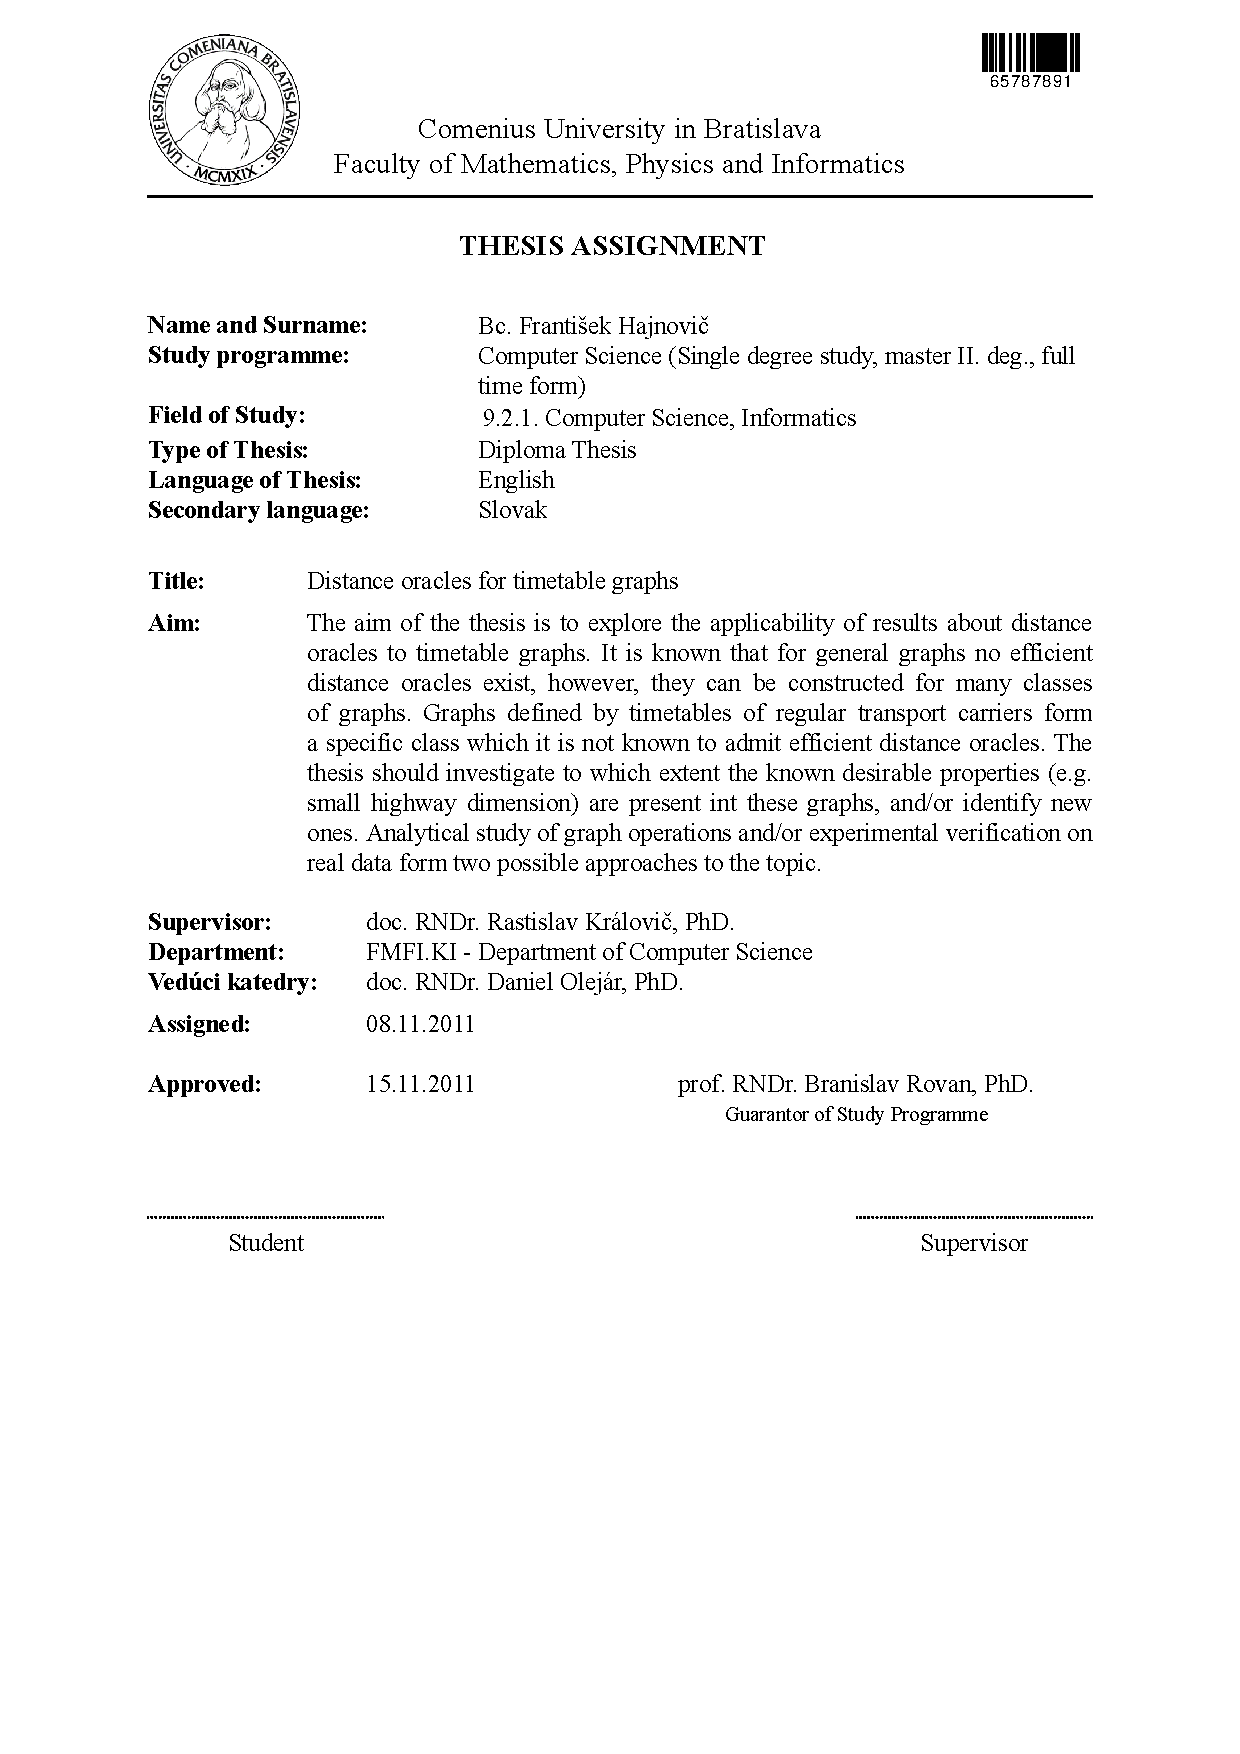
\includepdf[pages={1}]{../assignment-eng.pdf}
    
    \pagebreak
    
    %---------------------------------------------------------------------
    %   assignment
    %---------------------------------------------------------------------
	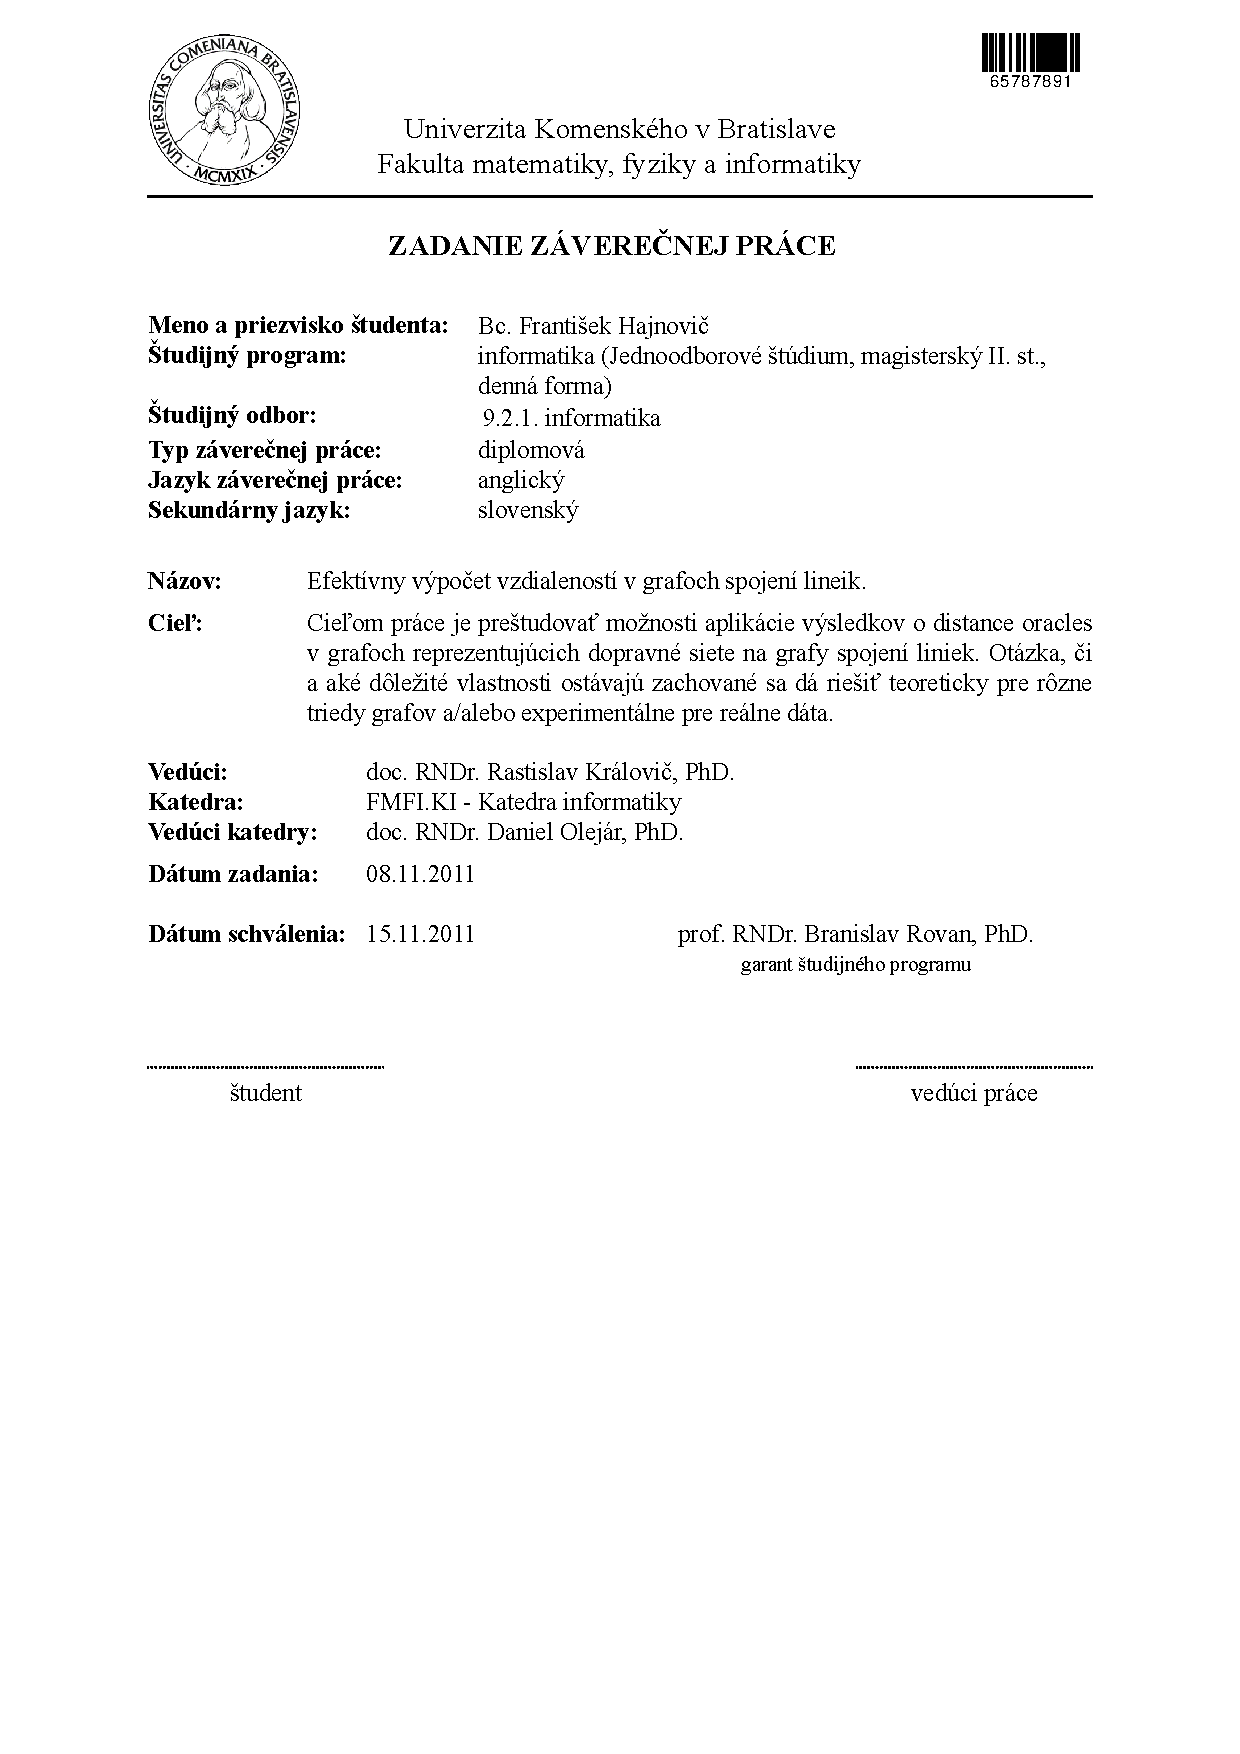
\includepdf[pages={1}]{../assignment-sk.pdf}
    
    \pagebreak

    %---------------------------------------------------------------------
    %   declaration of honesty
    %---------------------------------------------------------------------
    {~}\vfill

    I hereby declare that I wrote this thesis by myself, only with the help of the referenced literature, under the careful supervision of my thesis advisor.
    \vskip 1cm
    \hfill ............................

    \pagebreak

    %---------------------------------------------------------------------
    %   acknowledgements
    %---------------------------------------------------------------------
    \section*{Acknowledgements}
    I would like to thank ...

    \pagebreak

    %---------------------------------------------------------------------
    %   abstract
    %---------------------------------------------------------------------
    \begin{abstract}{Abstract}
        This thesis... \\

		Key words: \textbf{oracles}, \textbf{timetable}
	\end{abstract}	

    \begin{abstract}{Abstrakt}
        V tejto pr�ci...\\

		Kl��ov� slov�: \textbf{oracles}, \textbf{timetable}
	\end{abstract}	
	
    \pagebreak

    %---------------------------------------------------------------------
    %   contents
    %---------------------------------------------------------------------

    \tableofcontents

    \pagebreak

%---------------------------------------------------------------------
%   MAINMATTER  ------------------------------------------------------
%---------------------------------------------------------------------
    %\mainmatter
    \pagestyle{plain}
    \setcounter{page}{1}
    \setlength{\parindent}{40pt}

    %---------------------------------------------------------------------
    %   introduction
    %---------------------------------------------------------------------
    \section{Introduction}
    \label{sec:intro}
    \input parts/introduction.tex
    \pagebreak
   
    %---------------------------------------------------------------------
    %   preliminaries
    %---------------------------------------------------------------------
    \section{Preliminaries}
    \label{sec:prel}
    \input parts/preliminaries.tex
    \pagebreak
    
    %---------------------------------------------------------------------
    %   related work
    %---------------------------------------------------------------------
    \section{Related work}
    \label{sec:relwrk}
    \input parts/relatedwrk.tex
    \pagebreak
    
    %---------------------------------------------------------------------
    %   data
    %---------------------------------------------------------------------
    \section{Data \& analysis}
    \label{sec:data}
    \input parts/data.tex
    \pagebreak
    
    %---------------------------------------------------------------------
    %   usp
    %---------------------------------------------------------------------
    \section{Underlying shortest paths}
    \label{sec:usp}
    \input parts/usp.tex
    \pagebreak
    
    %---------------------------------------------------------------------
    %   neural
    %---------------------------------------------------------------------
    \section{Neural network approach}
    \label{sec:neural}
    \input parts/neural.tex
    \pagebreak
    
    %---------------------------------------------------------------------
    %   ttblazer
    %---------------------------------------------------------------------
    \section{Application TTBlazer}
    \label{sec:ttblazer}
    \input parts/ttblazer.tex
    \pagebreak

    %---------------------------------------------------------------------
    %   conclusion
    %---------------------------------------------------------------------
    \section{Conclusion}
    \label{sec:concl}
    \input parts/conclusion.tex
    \pagebreak
    
    %---------------------------------------------------------------------
    %   appendices
    %---------------------------------------------------------------------
    \begin{appendices}
  		\section{File formats}
  		\label{app:formats}
  		\input parts/formats.tex
	\end{appendices}
	\pagebreak

%---------------------------------------------------------------------
%   BACKMATTER  ------------------------------------------------------
%---------------------------------------------------------------------
    %\backmatter

    %---------------------------------------------------------------------
    %   bibliography
    %---------------------------------------------------------------------

    \bibliographystyle{is-alpha}
    %compile latex, bibtex, latex, latex
    \bibliography{../bibl}{}
\end{document} 